%%%%% START PREAMBLE HEADER %%%%%

%%% START REQUIRED PACKAGES %%%

\documentclass{article}
\usepackage[a4paper, total={7.25in, 9.5in}]{geometry} 
\usepackage{multirow}
\usepackage{lipsum}
\usepackage{hyperref}
\usepackage{listings}
\usepackage{graphicx}
\usepackage[table,xcdraw]{xcolor}
\usepackage[export]{adjustbox}
%\usepackage[superscript,biblabel]{cite}
\usepackage{amsmath}
\hypersetup{colorlinks=true,linkcolor=blue,filecolor=magenta,urlcolor=cyan,citecolor=blue}

%%% END REQUIRED PACKAGES %%%                


%%% START NEW COMMANDS new (shortcut) %%%

% This is a paragraph with normal font
\newcommand{\np}[1]{\paragraph*{\normalfont{#1}}}
% This is a text with a color
\newcommand{\ct}[2]{\textcolor{#1}{#2}}
% This is a bold text 
\newcommand{\bt}[1]{\textbf{#1}}
% This is an italic text 
\newcommand{\et}[1]{\emph{#1}}
% This is an underline text 
\newcommand{\ut}[1]{\underline{#1}}
% This is a newline shortcut
\newcommand{\n}{\\}
% This is a numbered equation with break line shortcut
\newcommand{\necbreak}[1]{\begin{equation}\begin{aligned}#1\end{aligned}\end{equation}}
% This is a numbered equation with break line shortcut
\newcommand{\nec}[1]{\begin{equation}#1\end{equation}}
% This is an equation shortcut
\newcommand{\ec}[1]{\begin{center} $#1$ \end{center}}
% Table title with bold text and correct space%
\newcommand{\titleTable}[2]{\np{\bt{Table #1} #2}}% Graph title with bold text and correct space%
\newcommand{\titleGraph}[2]{\np{\bt{Graph #1} #2}}
% Table body with border %
\newcommand{\bodyTable}[2]{\begin{center} \begin{tabular}{|#1|} \hline #2 \hline \end{tabular} \end{center} }
%%% END NEW COMMANDS (shortcuts) %%%


%%% START TITLE SETTINGS %%%
\title{\bt{Examen parcial Fisicoquímica de Sistemas Moleculares Organizados}}
\author{Pérez Alvarado Luis Raymundo, School of Chemistry, UNAM}
\date{04/12/2020}
%%% END TITLE SETTINGS %%%

%%%%% END PREAMBLE HEADER %%%%%

%%%%%%%%%%%%%%%% START DOCUMENT %%%%%%%%%%%%%%%%
\begin{document}

    \maketitle

    % Pregunta 1 %
    \np{1) Una molécula de L-Ala es colocada con su centro quiral en el origen de un sistema cartesiano dextrogiro. El átomo de carbono del carbonilo tiene las coordenadas atómicas [0, 0.15 cos(35.2°), -0.15 sen(35.2°)] y el carbono C$\beta$ (grupo metilo) en [0, -0.15 cos(35.2°), -0.15 sen(35.2°)].}


    \begin{itemize}
        \item Muestre como se determinaron las coordenadas y y z para el carbono del carbonilo y el carbono C$\beta$ del grupo metilo. Considere que la longitud del enlace sencillo C–C es de 0.15 nm.
        \item En ese mismo sistema de coordenadas determine las coordenadas (x, y, z) para el nitrógeno y
        el hidrógeno del grupo amino. Emplee un valor de longitud de enlace C–H de 0.11 nm y C–N
        de 0.13 nm.
        \item Escriba el operador que genere las coordenadas para D-Ala.
        \item ¿Cuáles son las coordenadas para estos mismos átomos en D-Ala?
    \end{itemize}


     % Pregunta 2 %
     \np{2) Un residuo de amino ácido es colocado con su carbono C$\alpha$ en las coordenadas (0, 0.23, 0.05)nm en un sistema cartesiano dextrogiro.}

     \begin{itemize}
        \item Calcule las coordenadas para todos los carbonos C$\alpha$ de seis residuos de amino ácido en la
        conformación extendida con el eje y como el eje helicoidal.
        \item Calcule las coordenadas para todos los carbonos C$\alpha$ de seis residuos de amino ácido en una
        $\alpha$-hélice, con el eje z como su eje helicoidal. (El radio de la $\alpha$-hélice es de 0.226 nm ).
    \end{itemize}

    \np{1) Se uso el programa gauss view y se estimó la distancia en amstrongs que hay entre un carbono $\alpha$ y un carbono $\alpha$ en un enlace peptídico que es de 3.9 lo que es 0.39nm, considerando que se mueve la cadena de forma lineal sobre el eje y se puede usar el sigueinte operador de simetría traslacional para obtener las posiciones de los carbonos $\alpha$.}

    \ec{\hat{T}(x,y,z)=(x',y',z')=(x,y+0.39,z)}

    \begin{center}
        \begin{tabular}{ |c|c| } 
            \hline
            Carbono $\alpha$ & Coordenada y (nm) \\ 
            \hline 
            1 & 0.23\\
            \hline 
            2 & 0.62\\
            \hline 
            3 & 1.01\\
            \hline 
            4 & 1.40\\
            \hline 
            5 & 1.79\\
            \hline 
            6 & 2.18\\
            \hline 
        \end{tabular}
    \end{center}

    \np{2) Se construyó el siguiente operador helicoidal para poder contruir una hélice sobre el eje helicoidal y.}

    \ec{\hat{C}_{x-z}+T_y=(xCos(\theta)+zSen(\theta),y+\hat{T},xCos(\theta)+zSen(\theta))nm}

    \np{Con el operador de simetria usando como a c = 0.226m y considerando el operdor de traslación como 0.15nm (que fue la division del paso de la cuerda de una alfa helice entre 3.6 residuos) se pueden obtener las coordenas de los carbonos alfas a los que se les aplica el operador.}

    Donde \theta=2pi/0.226

    \ec{\hat{C}_{x-z}+T_y=(x(-0.89)-z(0.45),y+\hat{T},x(0.45)+z(-0.89))nm}
    
    \begin{center}
        \begin{tabular}{ |c|c|c|c| } 
            \hline
            Carbono $\alpha$ & y (nm) & x (nm) & z (nm)\\ 
            \hline 
            1 & 0.23 & 0 & 0.05\\
            \hline
            2 & 0.38 & -0.02 & -0.04\\
            \hline 
            3 & 0.53 & 0.03 & 0.01 \\
            \hline 
            4 & 0.68 & -0.03 & 0.005\\
            \hline 
            5 & 0.83 & 0.02 & -0.01\\
            \hline 
            6 & 0.98 & -0.02& 0.02 \\
            \hline 
        \end{tabular}
    \end{center}

    \np{Se redondearon los números, para apreciar la posición del carbono alfa.}

    % Pregunta 3 %
    \np{3) Dibuje la estructura del tripéptido Ser-Pro-Ala con el enlace peptídico Ser-Pro en la configuración cis, el otro enlace peptídico en la posición trans y todos los carbones C$\alpha$ en la conformaci ́on trans.}

    \begin{itemize}
        \item ¿Por qué cree que el enlace Ser-Pro se encuentra prefencialmente en la configuración cis en contra posición a la configuración trans que presentan otros enlaces peptídicos?
        \item ¿Cuál es la consecuencia estructural de colocar este enlace peptídico en la configuración cis?
    \end{itemize}

    \begin{figure}[h]
        % Reactive %
        \centering
        \begin{minipage}[b]{0.49\textwidth}
            \centering
          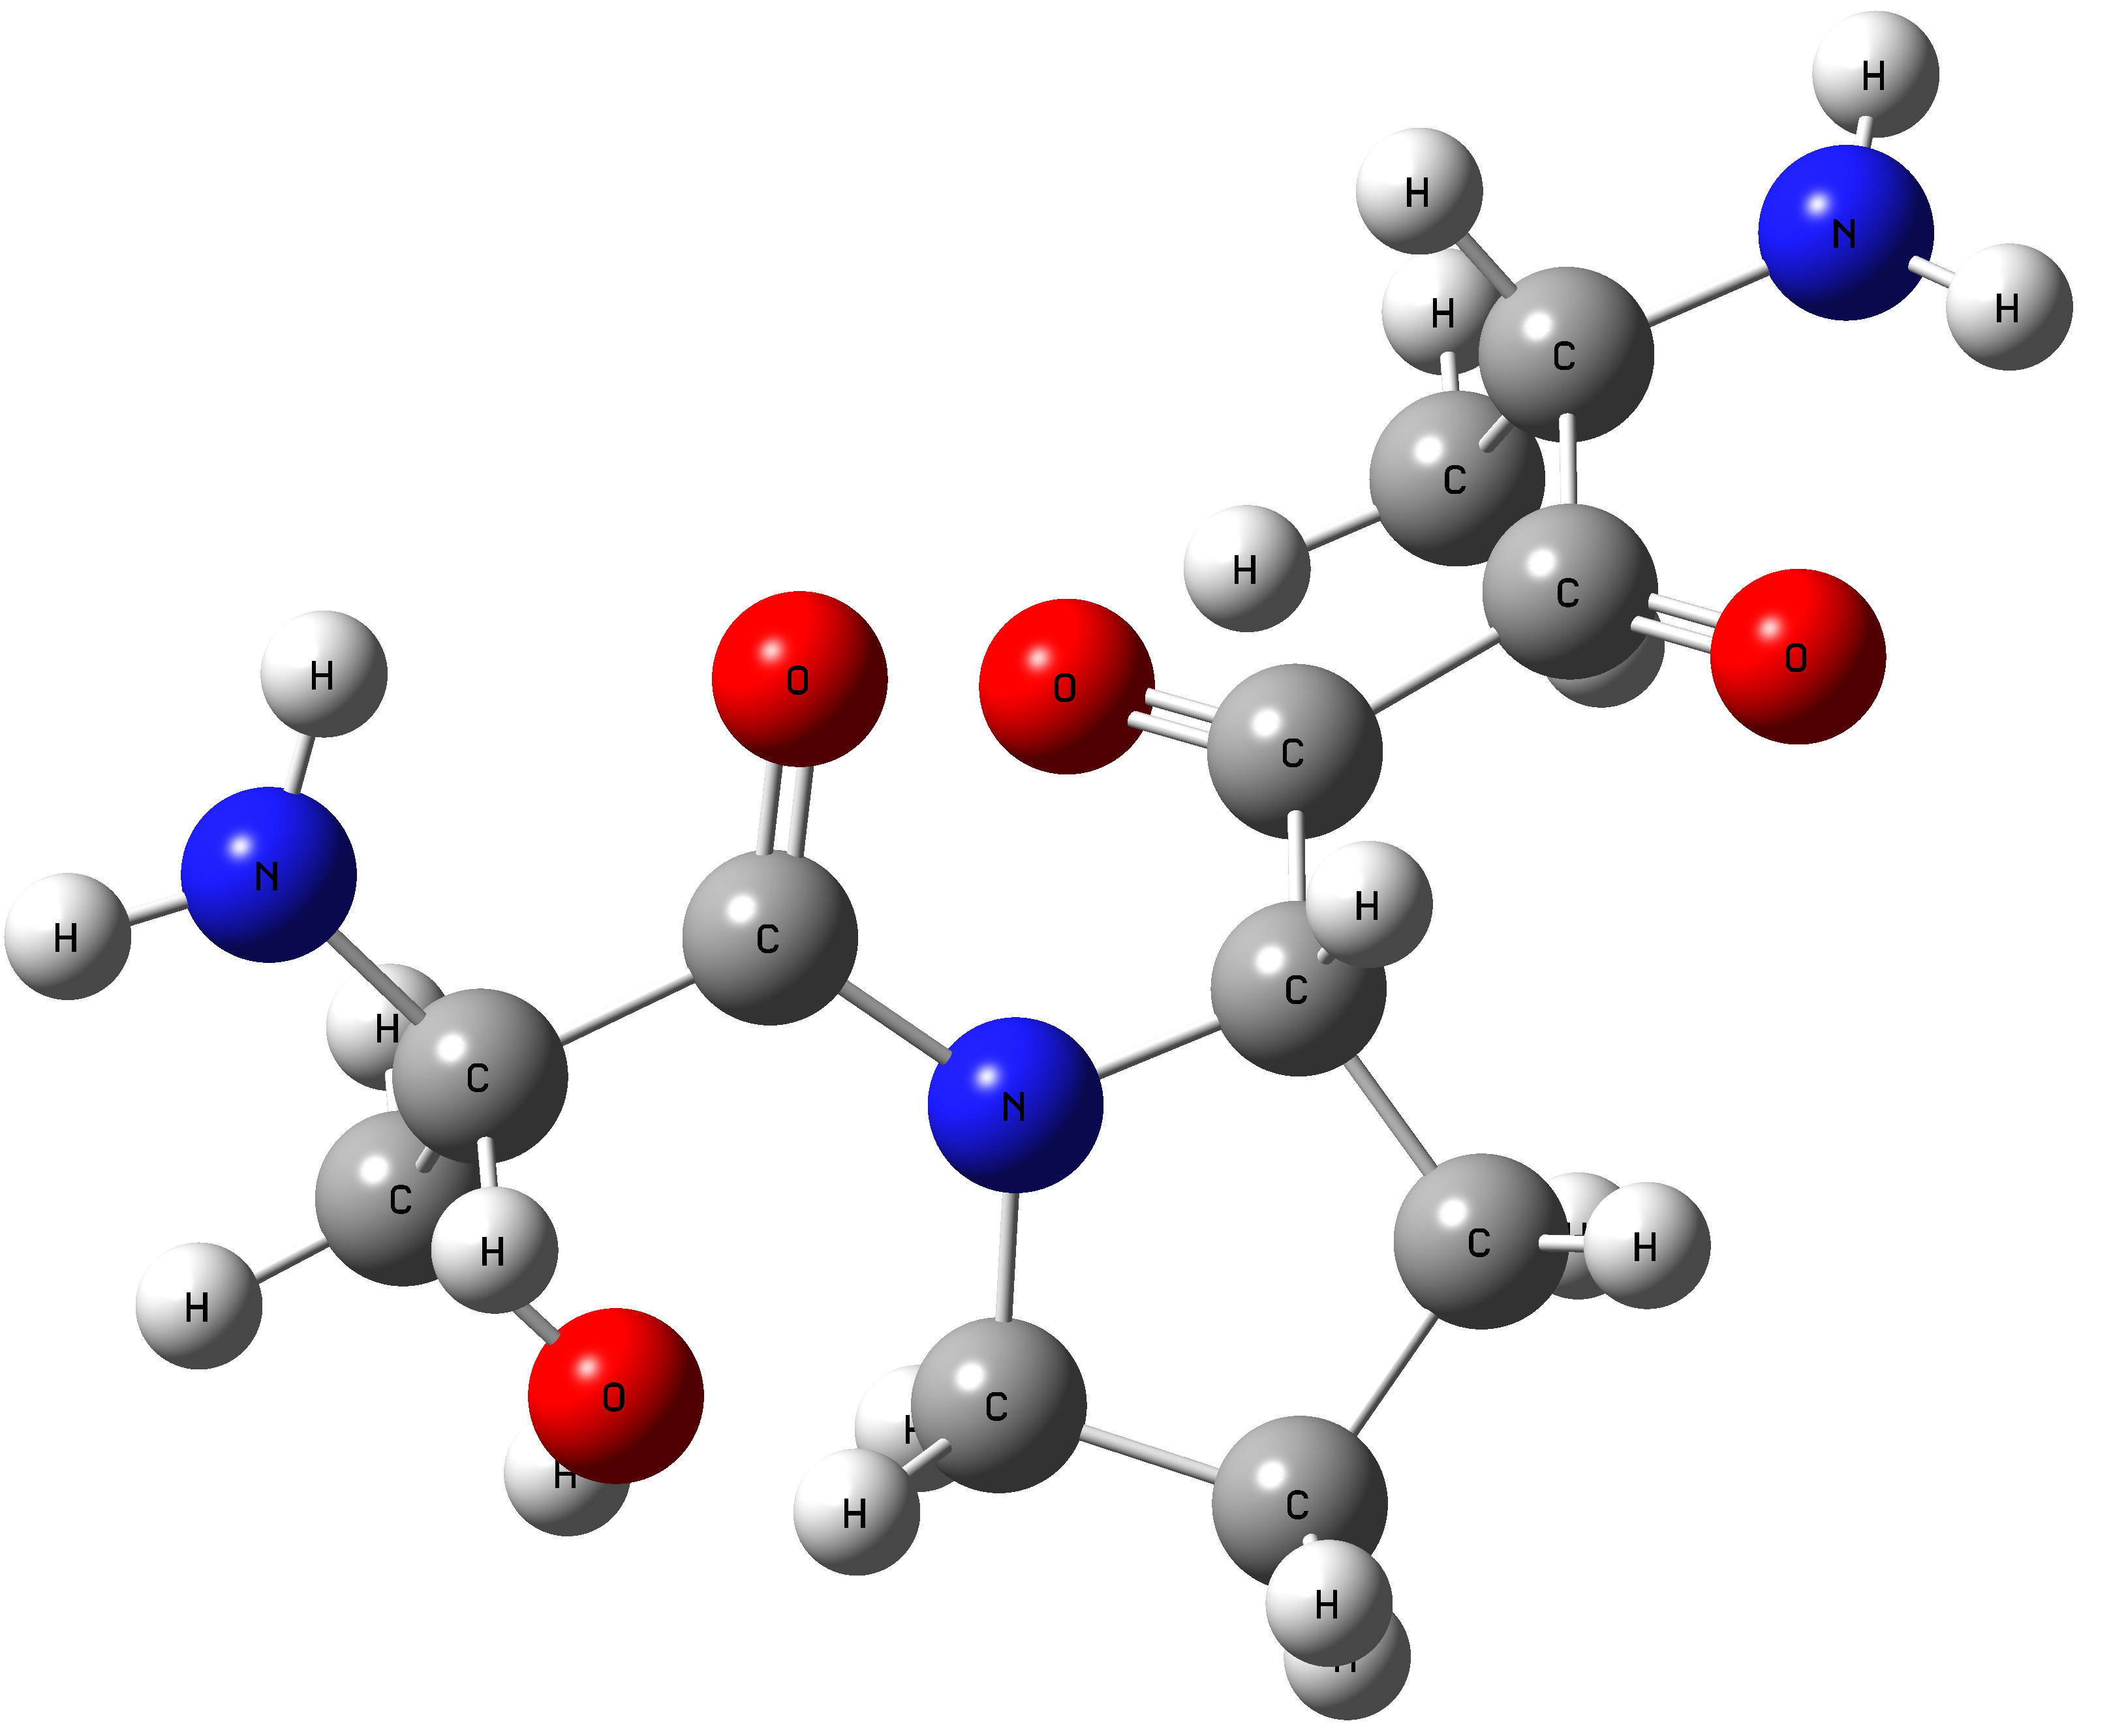
\includegraphics[scale=0.085]{triT.jpg}
          \caption{Tripéptido Trans.}
        \end{minipage}
        \begin{minipage}[b]{0.49\textwidth}
            \centering
          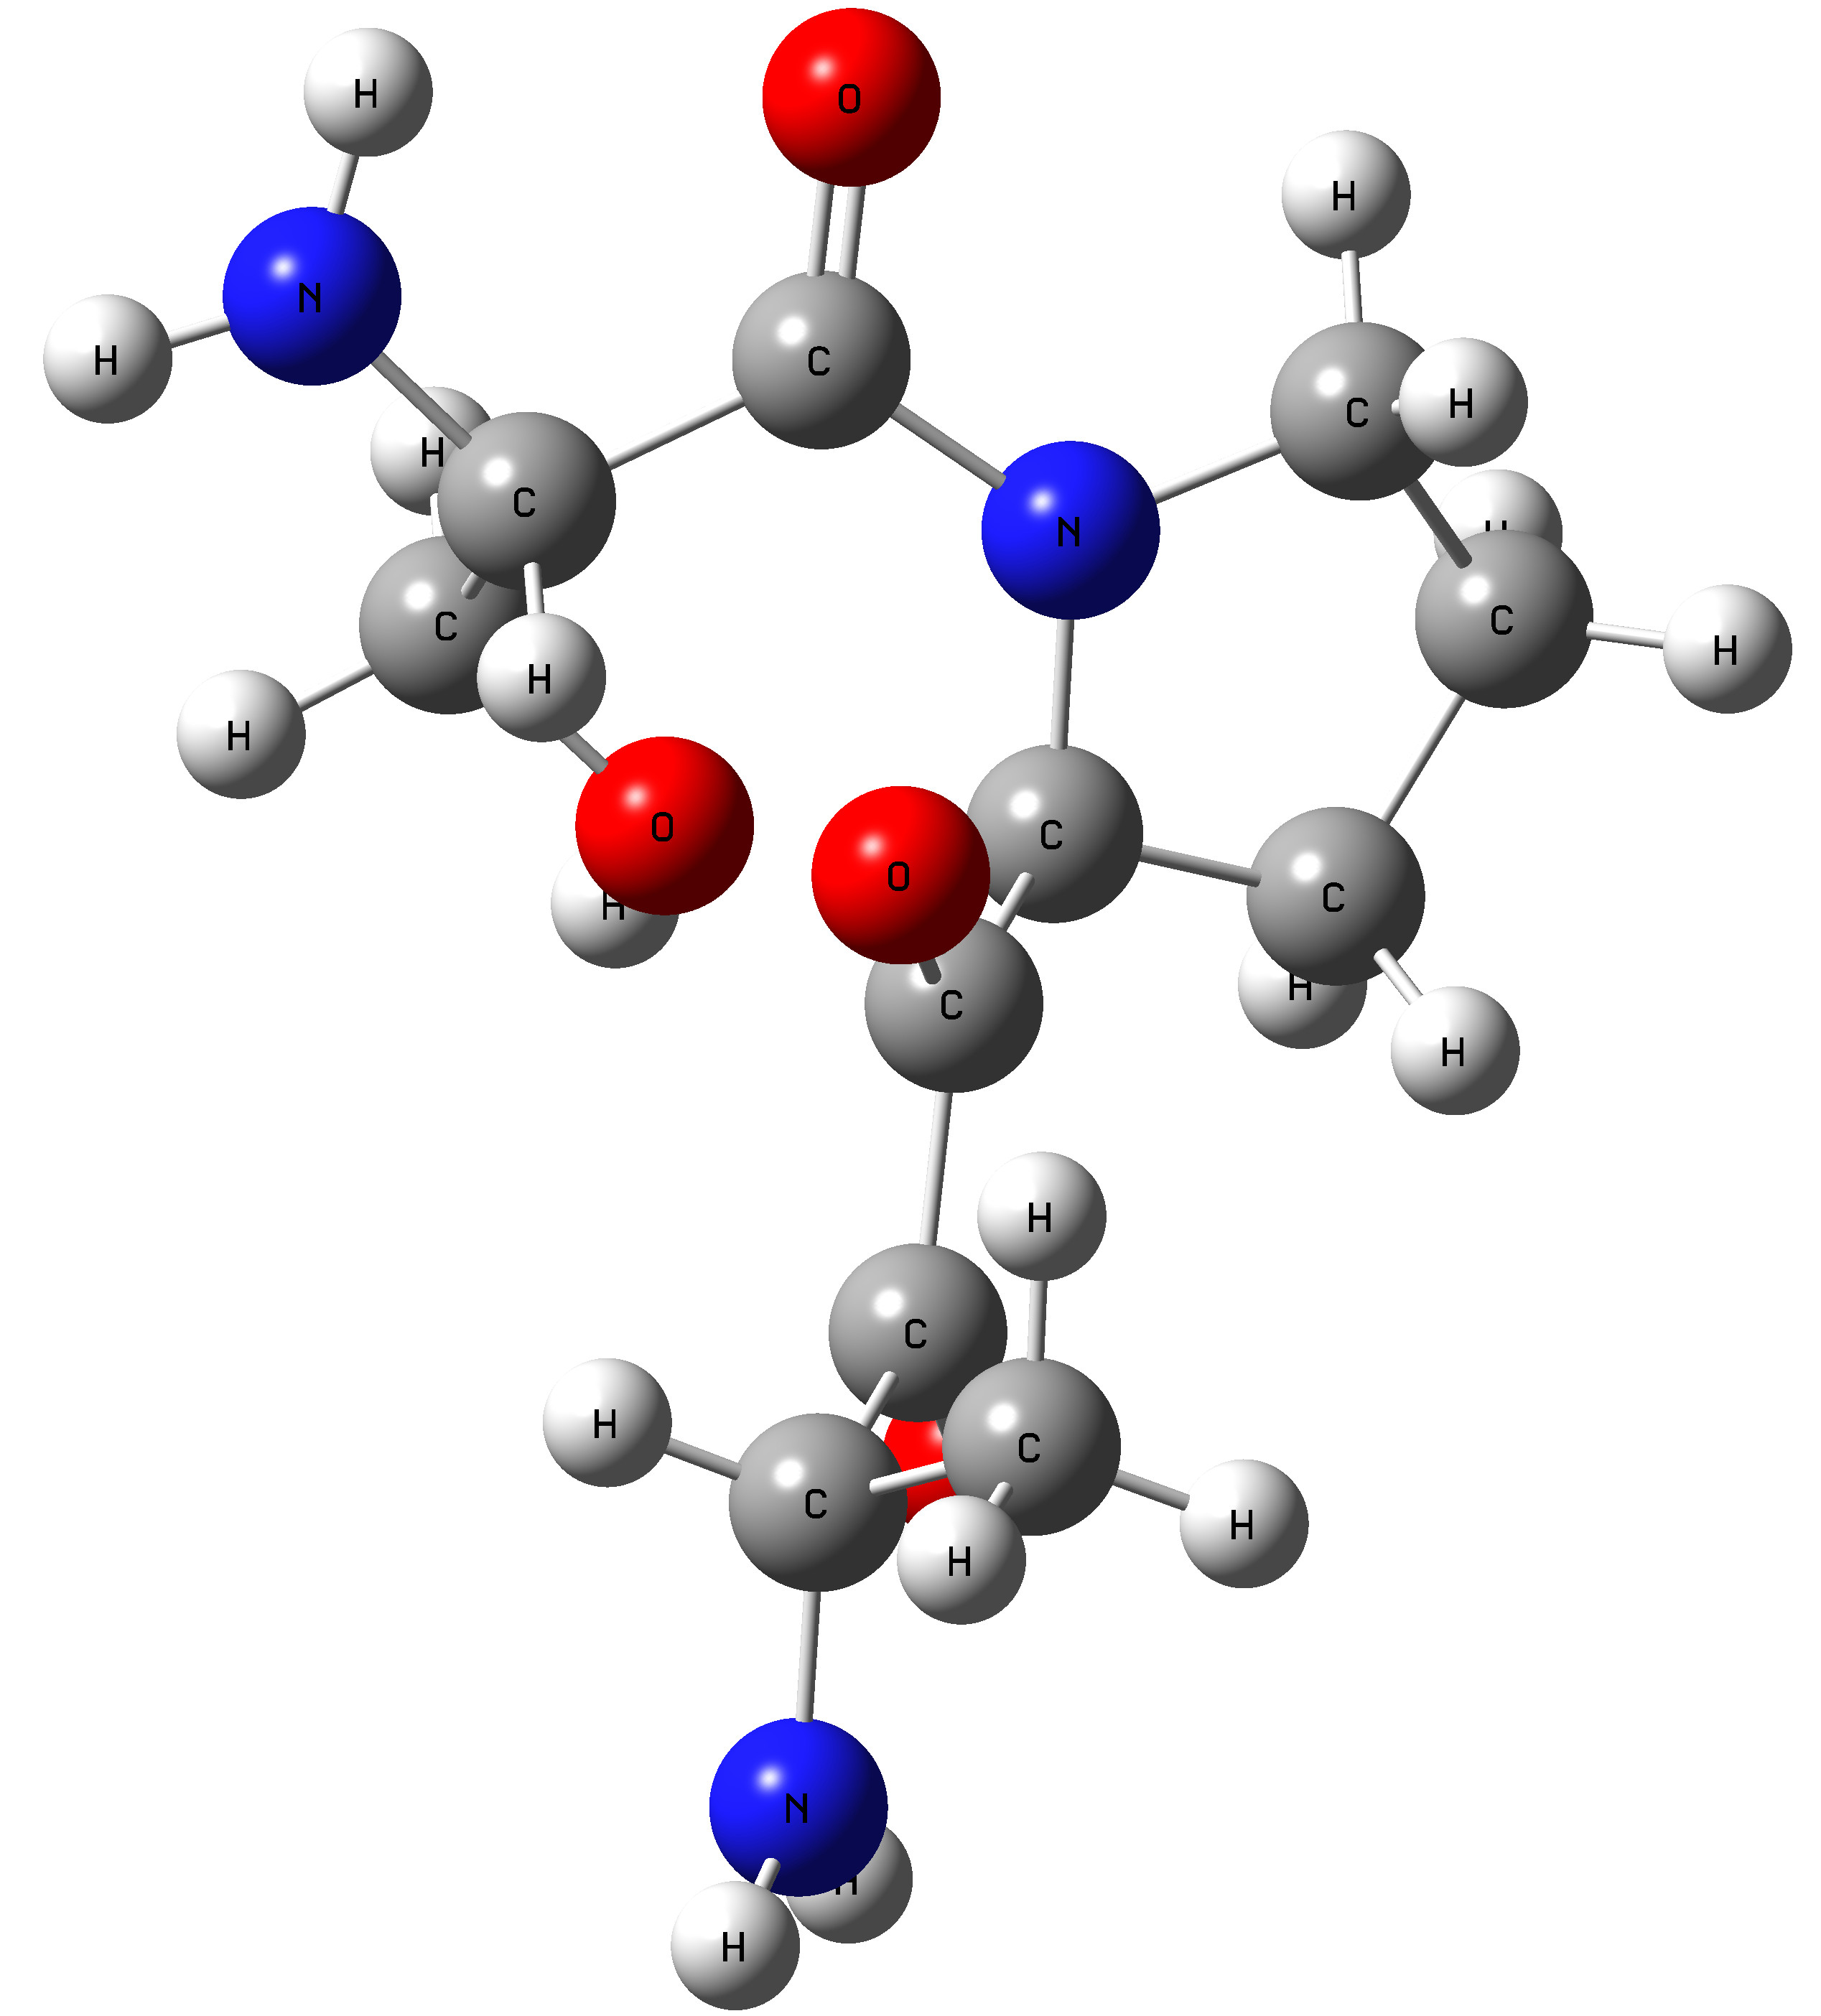
\includegraphics[scale=0.085]{triC.jpg}
          \caption{Tripéptido Cis.}
        \end{minipage}
        \begin{minipage}[b]{0.32\textwidth}
            \centering
          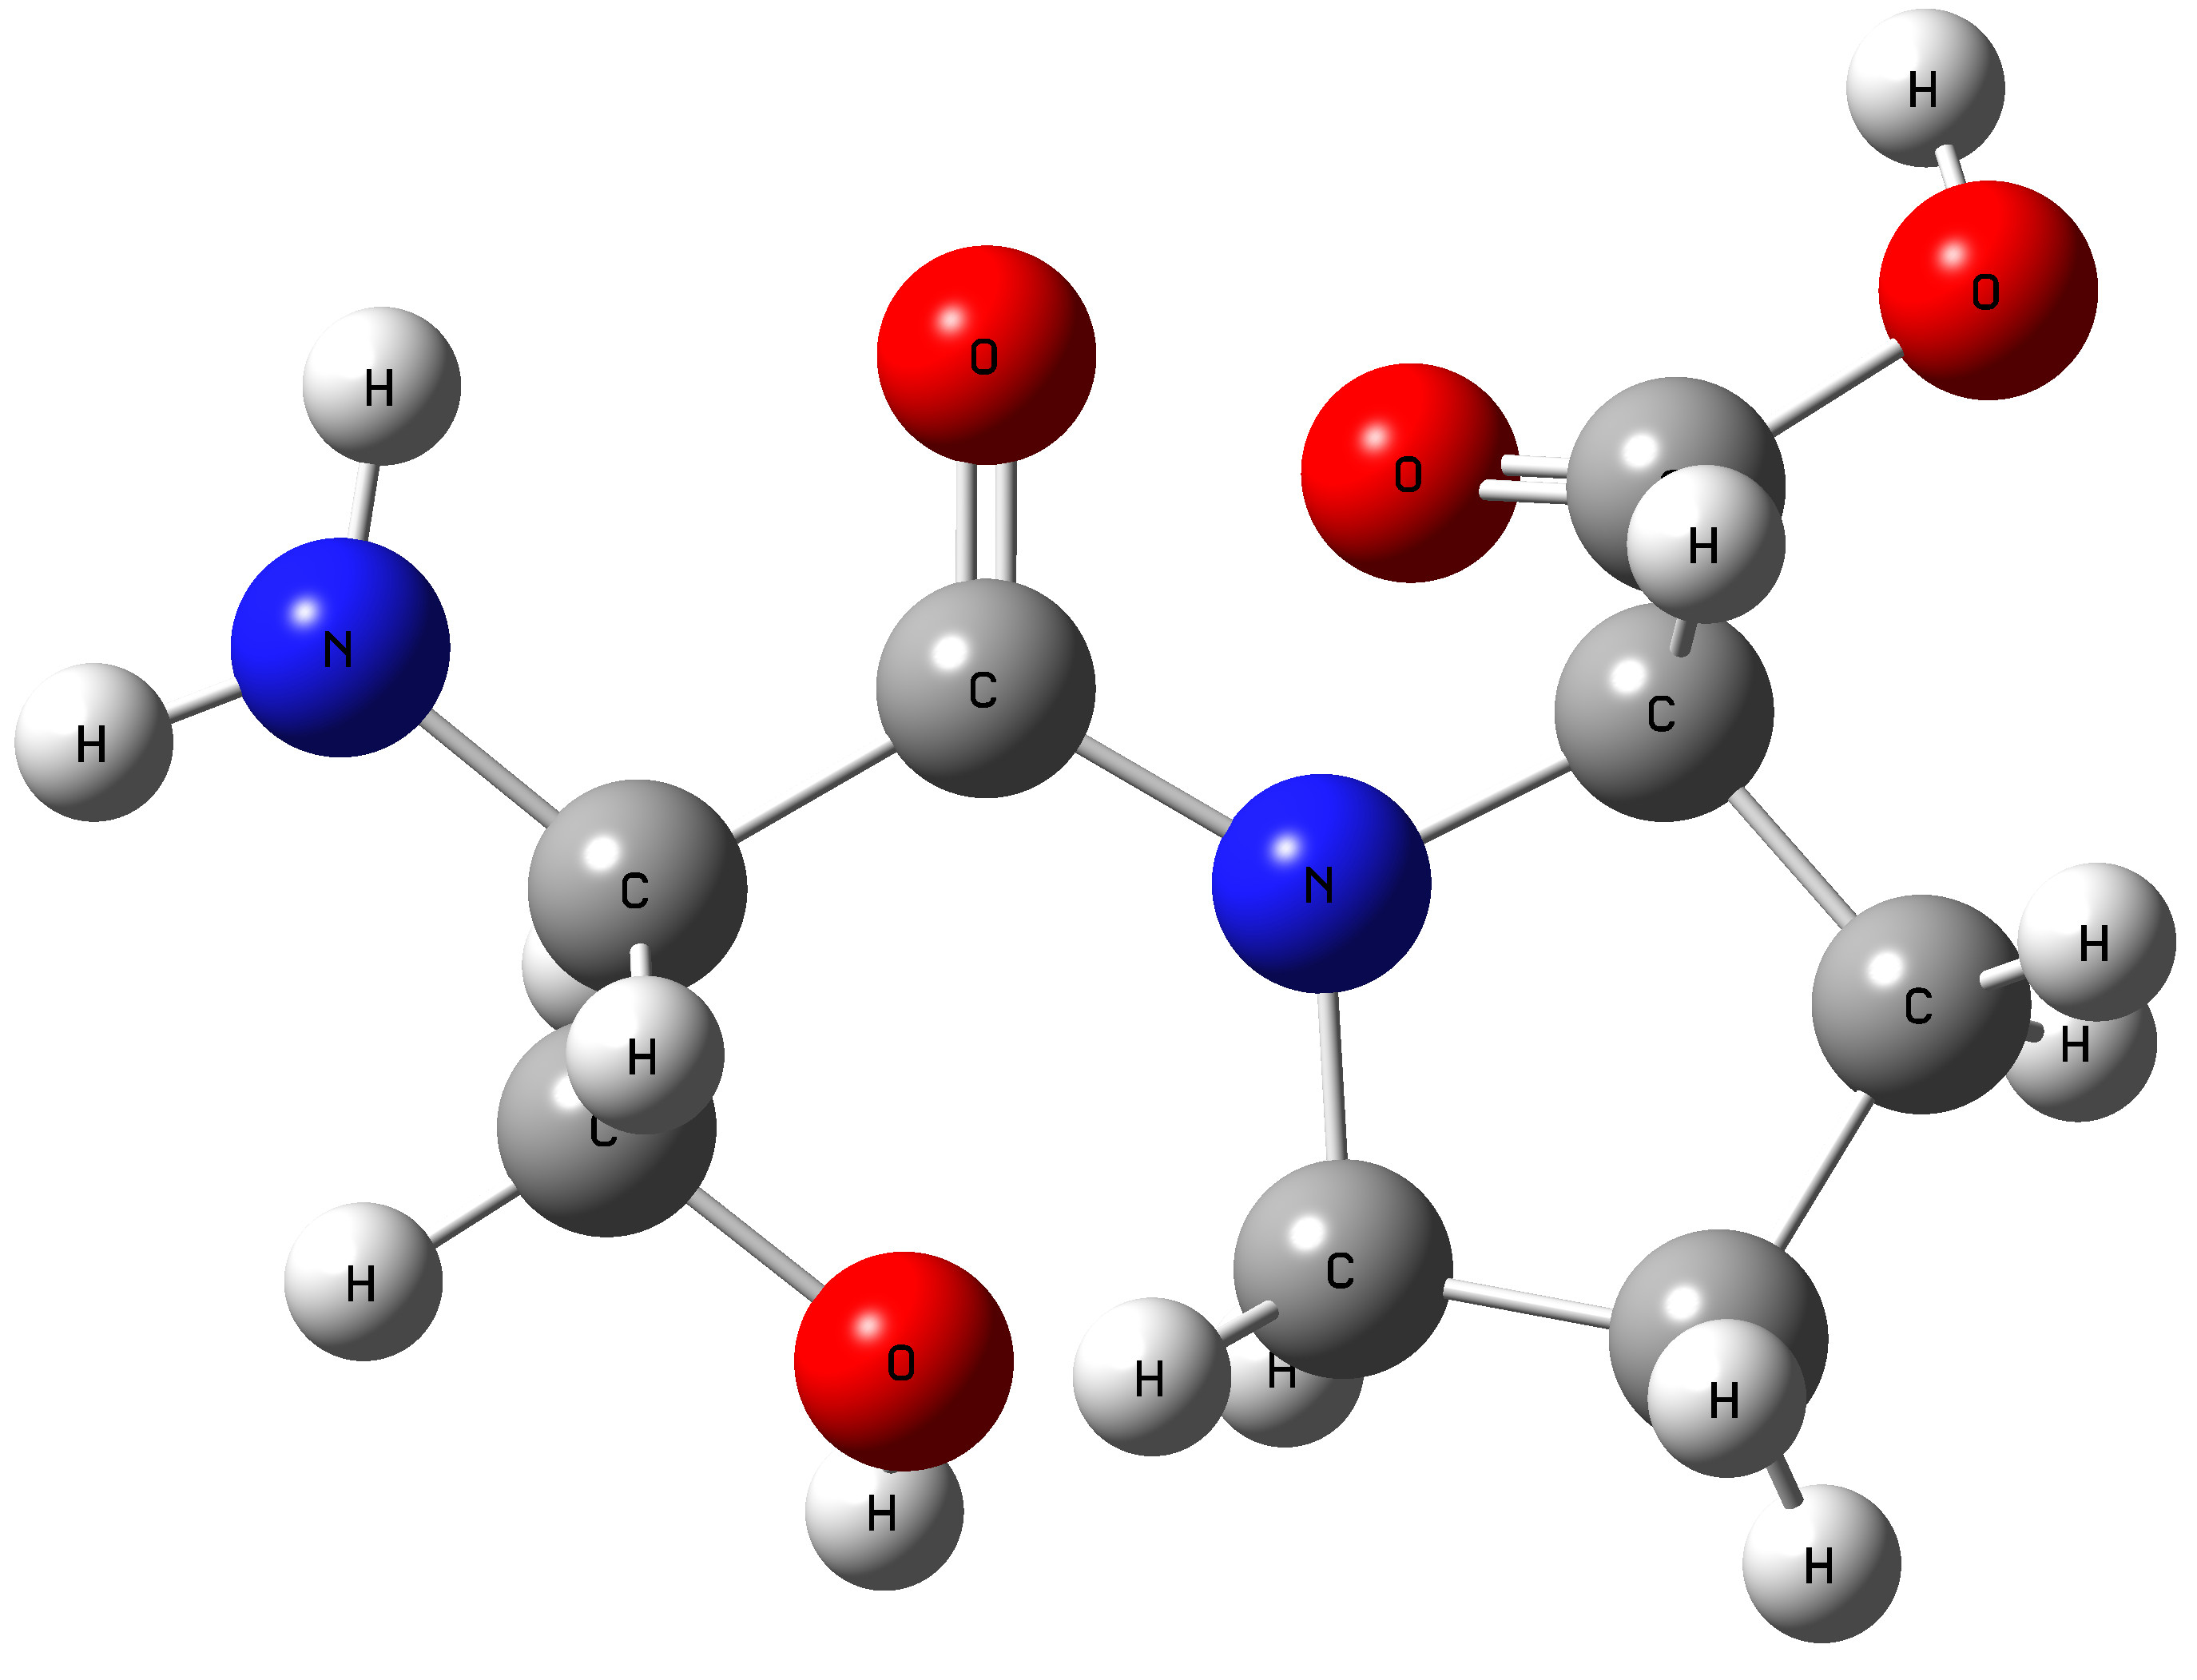
\includegraphics[scale=0.085]{tripeptidoTrans.jpg}
          \caption{Enlace peptídico Ser-Pro conformación trans.}
        \end{minipage}
        \hfill
        \begin{minipage}[b]{0.32\textwidth}
          \centering
          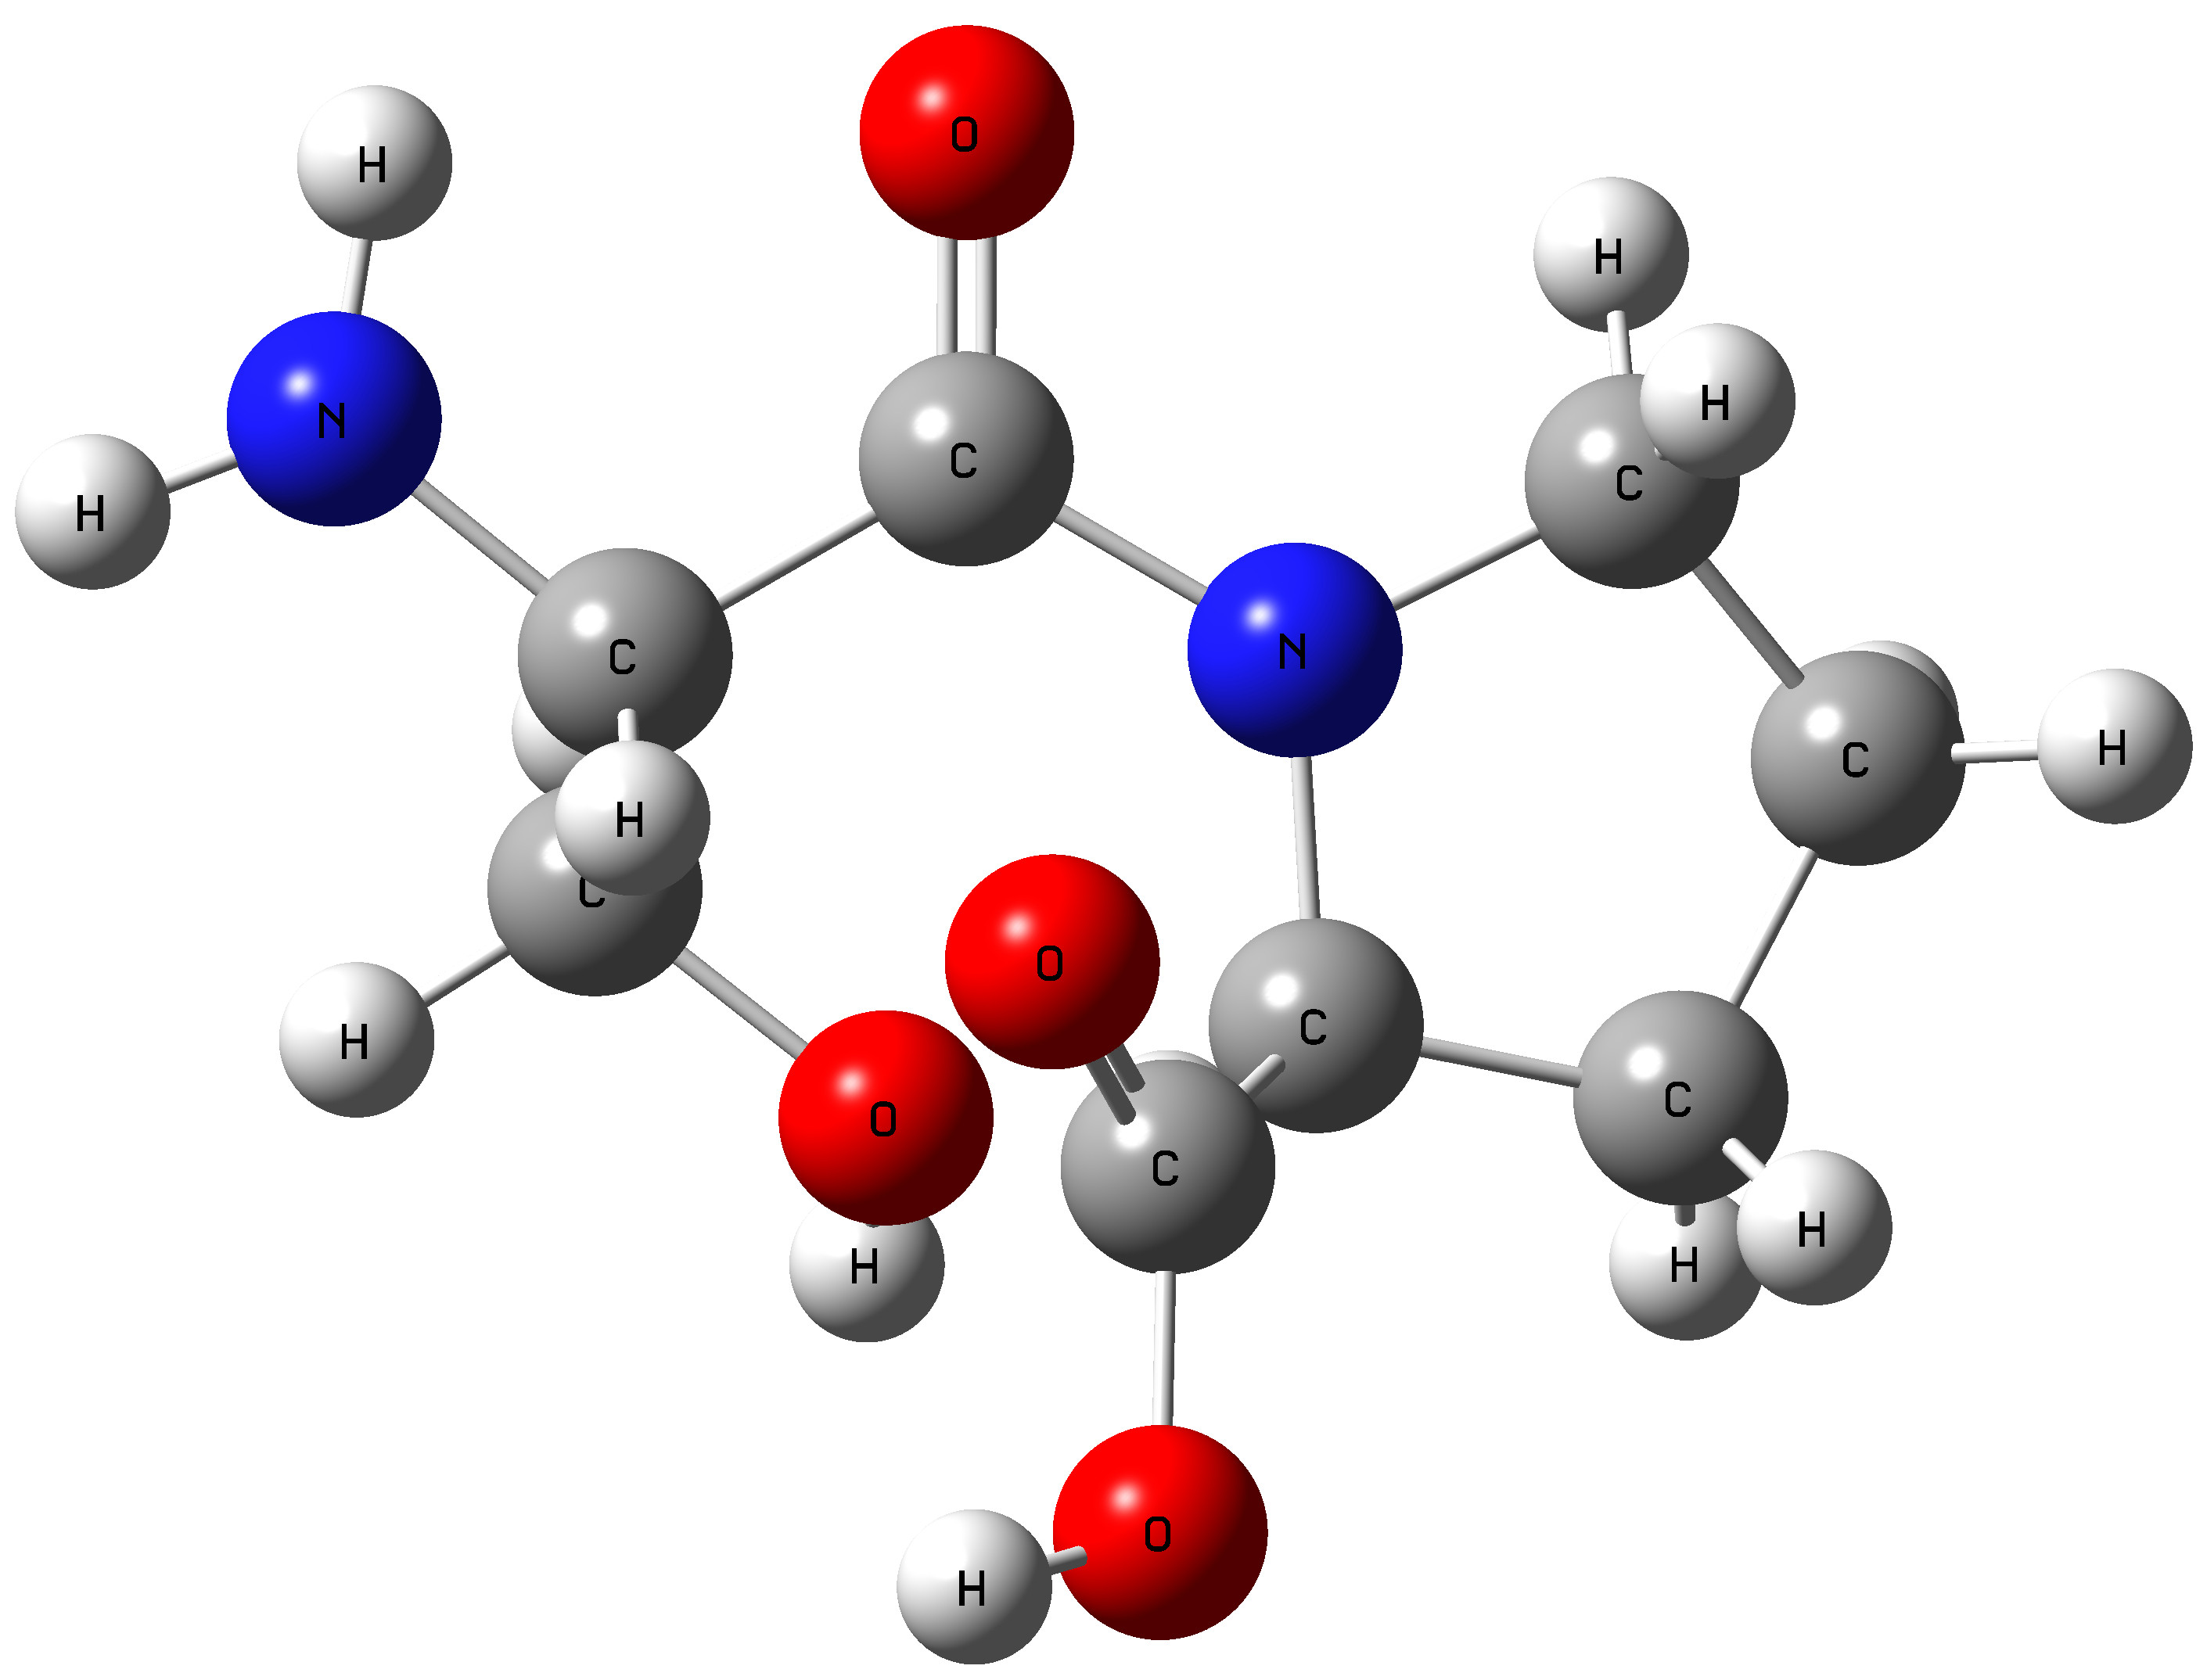
\includegraphics[scale=0.085]{tripeptidoCis.jpg}
          \caption{Enlace peptídico Ser-Pro conformación cis vista frontal.}
        \end{minipage} 
        \hfill
        \begin{minipage}[b]{0.32\textwidth}
          \centering
          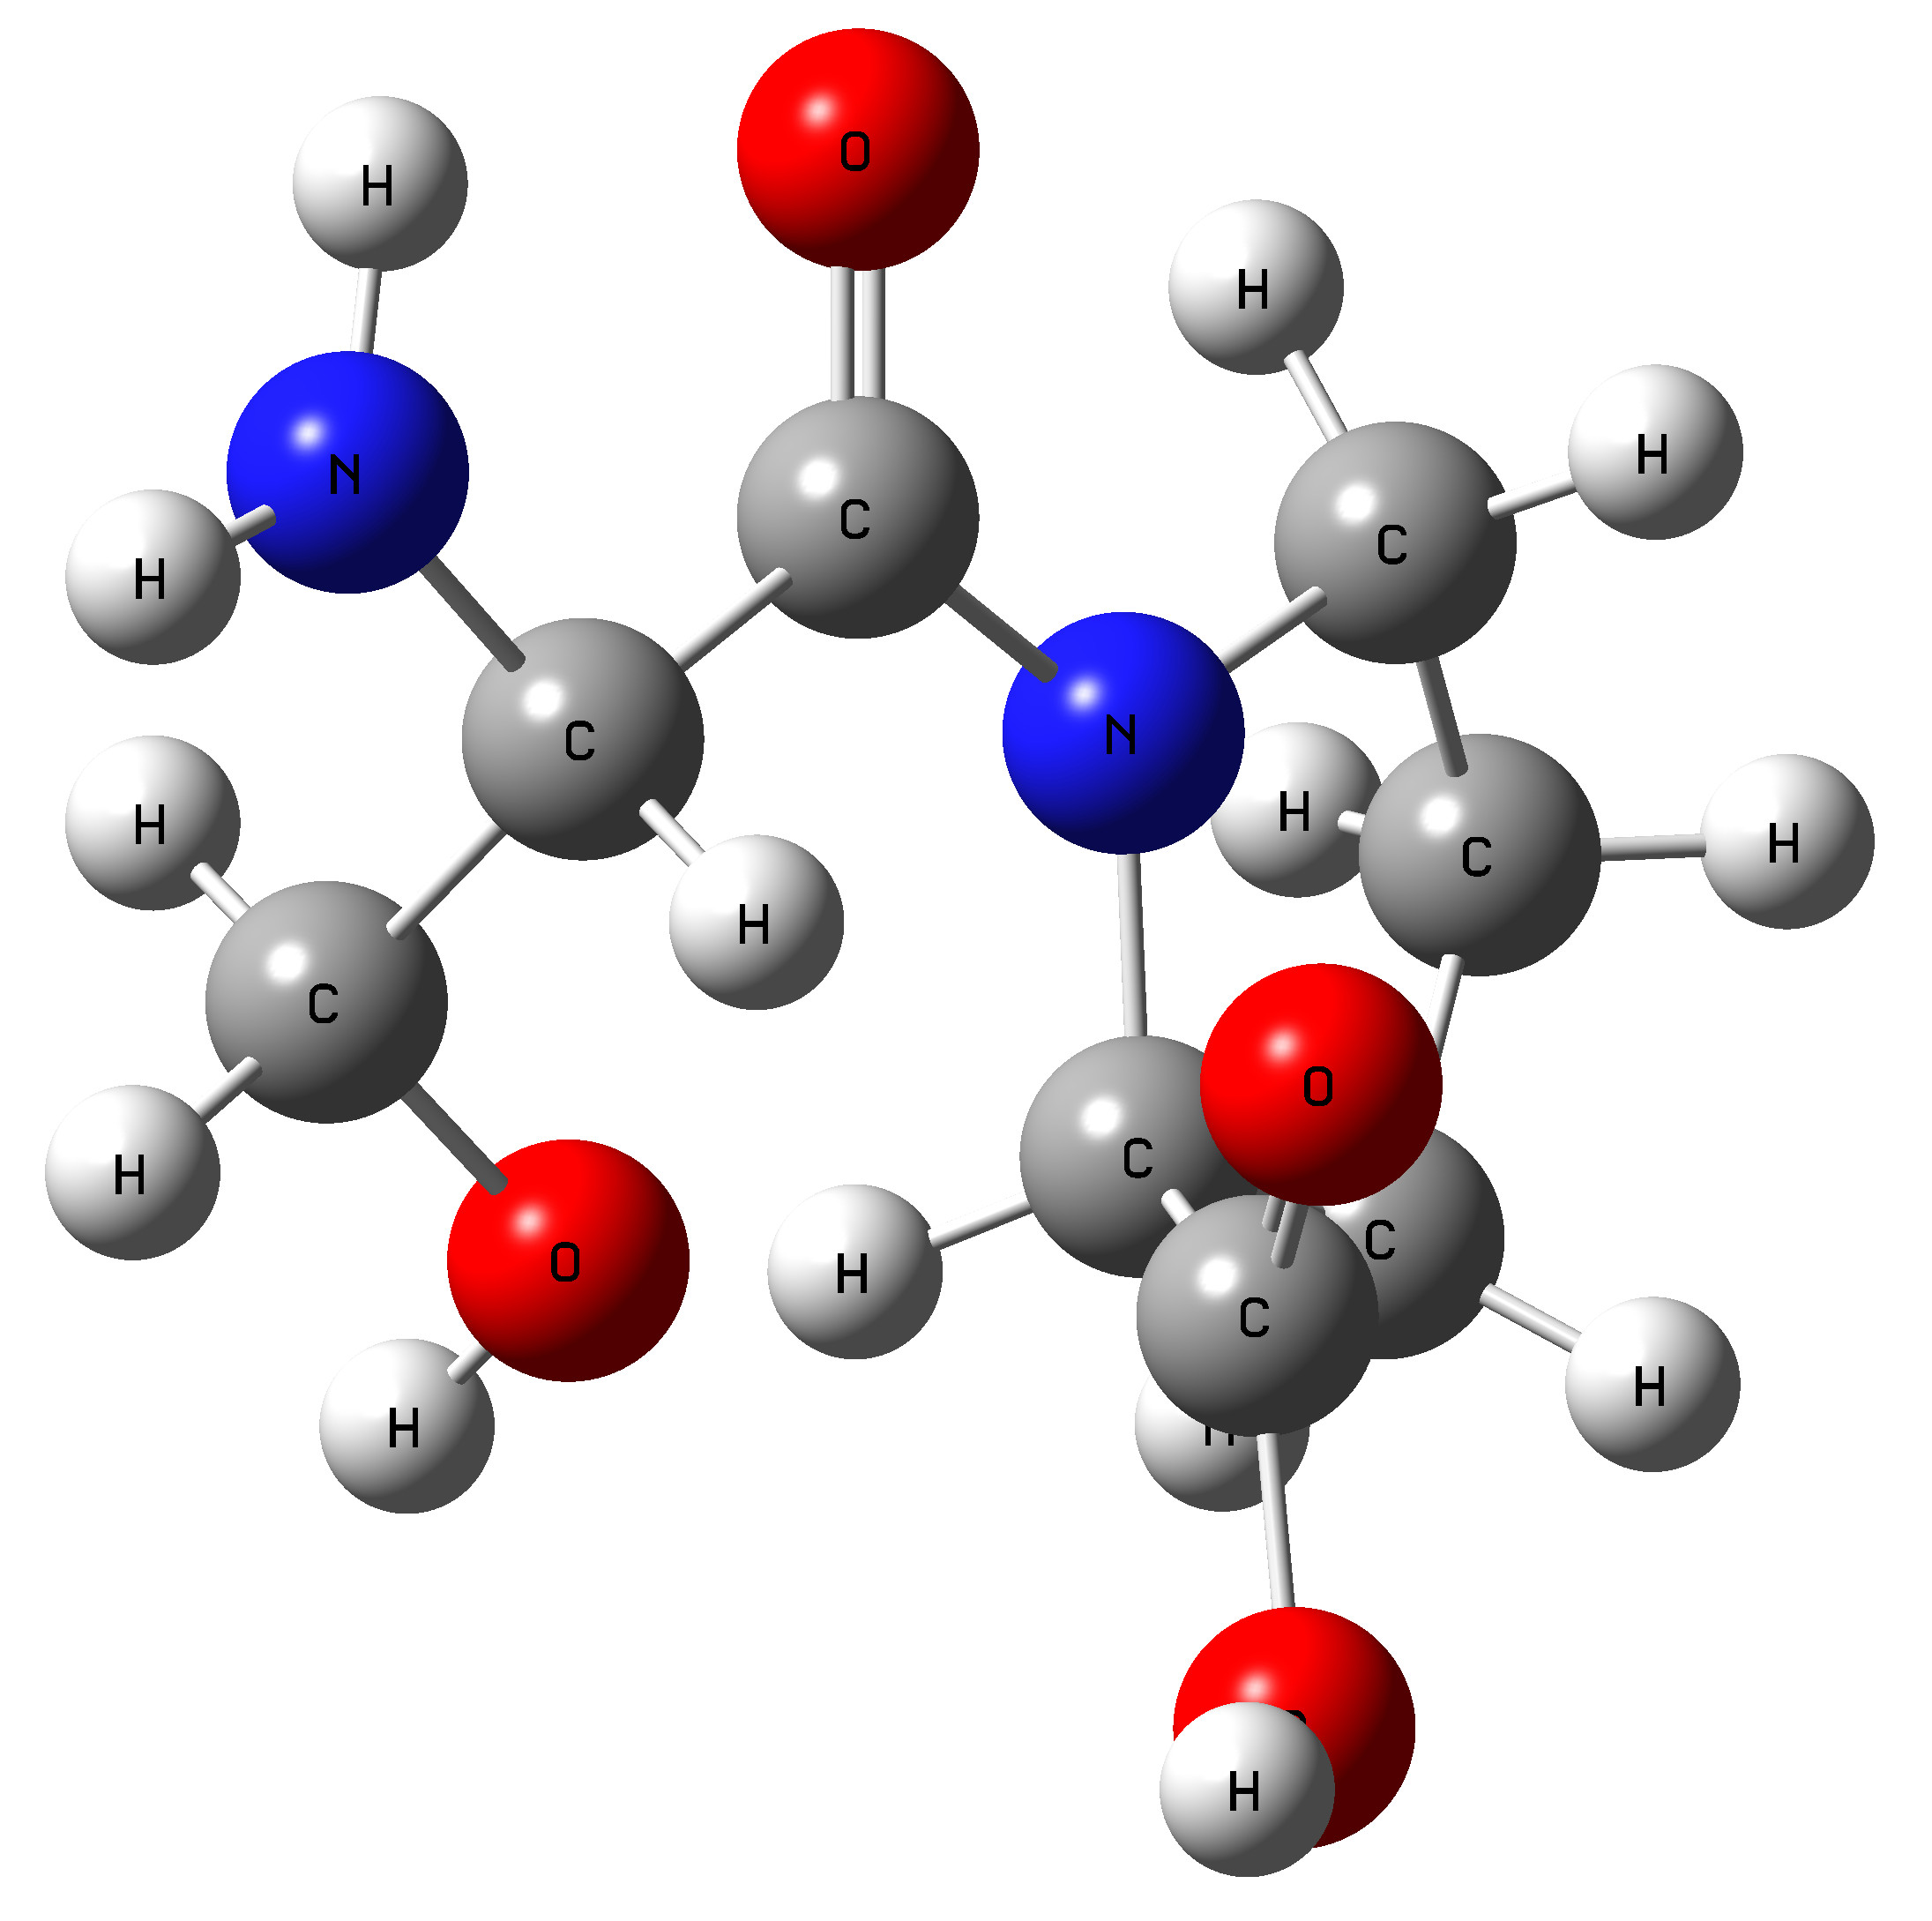
\includegraphics[scale=0.085]{tripeptidoCis2.jpg}
          \caption{Enlace peptídico Ser-Pro conformación cis vista vista lateral.}
        \end{minipage} 
    \end{figure}

    \np{1) La preferencia de la conformación cis cuando el segundo aminoácido del enlace peptídico es un residuo de prolina, es debido a que en ambas conformaciones hay impedimento estérico entre el carbono $\alpha$ del primer aminoácido y ya sea el carbono $\alpha$ en la posición cis y con el carbono $\gamma$ en la posición trans de la prolina, lo cual se observa en las figuras mostradas del enlace Ser-Pro, lo que da lugar a un equilibrio entre ambas conformaciones, y en la cual la mas estable es la conformación cis.}
    
    \np{Al observar su estructura 3D se puede sugerir que es debido a que en la posición trans además de los ipedimentos entre el carbono $\alpha$-$\alpha$ y $\alpha$-$\gamma$ hay impedimentro entre los átomos oxígenos que conforman los enlaces peptídicos, lo cual harian menos favorable dicha conformación (figura 1).}

    \np{2) El cambio estructural es que el carbonon $\alpha$ queda del mismo lado que el carbono $\gamma$ en lugar de $\alpha$  con el $\alpha$ como es en la conformación trans, además tiene como consecuencia que esta conformación produce un cambio en la dirección del péptido, y es responsable de que una cadena forme parte de los giros $\beta$, especificamente los giros de tipo II en donde uno de los cuatro residuos de aminoácidos que forman este giro es la prolina.}

    % Pregunta 4 %
    \np{4) En la figura 1 se muestra el gráfico de contactos entre amino ácidos para la prote ́ına tripsina, obtenida a partir de la estructura de un cristal (adaptado de Oas, T. G., Kim, P. S. (1988), Nature, 336, 42-48).}

    \begin{itemize}
        \item Asigne toda la estructura secundaria de la proteína.
        \item Realice un esquema de la estructura terciaria de la proteína, dando un arreglo aproximado de las $\alpha$-hélice y las hojas $\beta$.
    \end{itemize}

    \begin{figure}[h!]
        % Reactive %
        \centering
        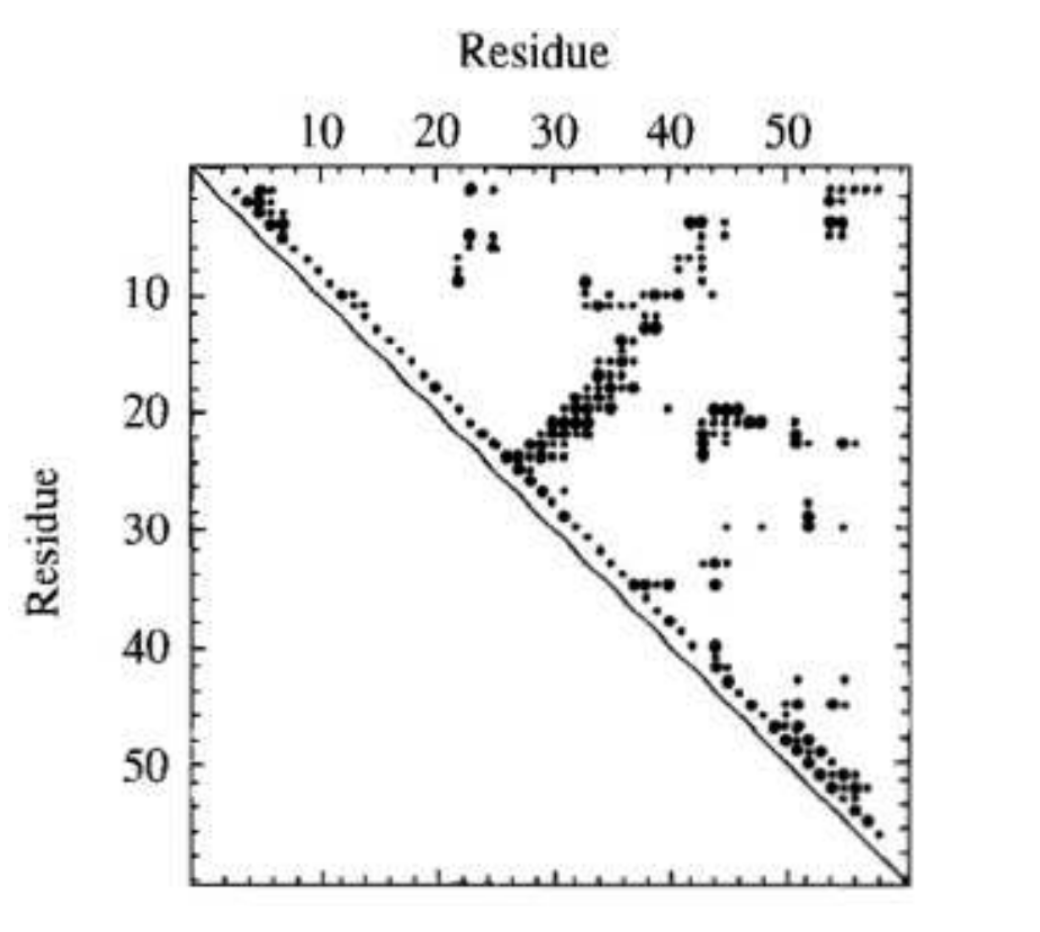
\includegraphics[scale=0.35]{grafico1.jpg}
        \caption{Gráfico de contactos entre amino ácidos para la proteína tripsina.}
    \end{figure}

    \np{1) Con el gráfico de contacto se puede observar una alfa helice del residuo 2 al 8,se aprecia una hoja beta antiparalela del residuo 26 al 40 , del 40 al 50 una posible hoja beta paralela y una hélice alfa del residuo 50 al 60. En la siguiente figura se observa un esquema de la estructura secundaria.}
    
    \np{2) En en esquema realizado se puede apreciar la estructura secundaria basada en el gráfico de contacto de una sección de la tripsina.}

    \begin{figure}[h!]
        % Reactive %
        \centering
        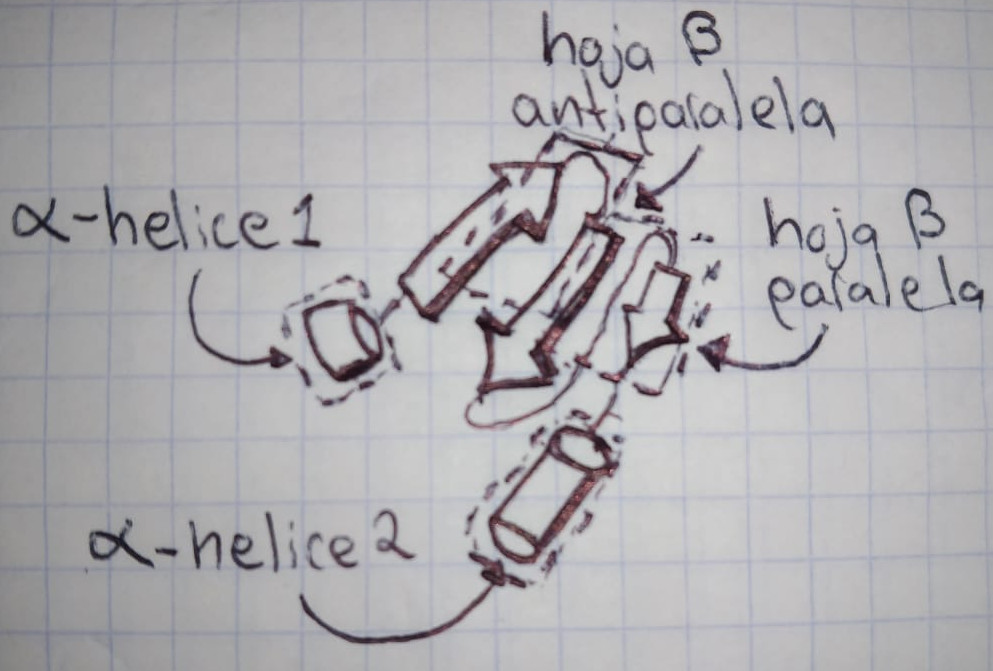
\includegraphics[scale=0.85,frame]{esquema.jpg}
        \caption{Dibujo de la estructura secundaria de una sección de la tripsina.}
    \end{figure}

    % Pregunta 5 %
    \np{5) Realice un gráfico de contactos, que muestre los contactos entre aminoácidos para un meandro $\beta$, formado por tres hebras, con seis residuos de aminoácido en cada hebra y cuatro residuos de aminoácidos en los giros.}

    \begin{figure}[h!]
        % Reactive %
        \centering
        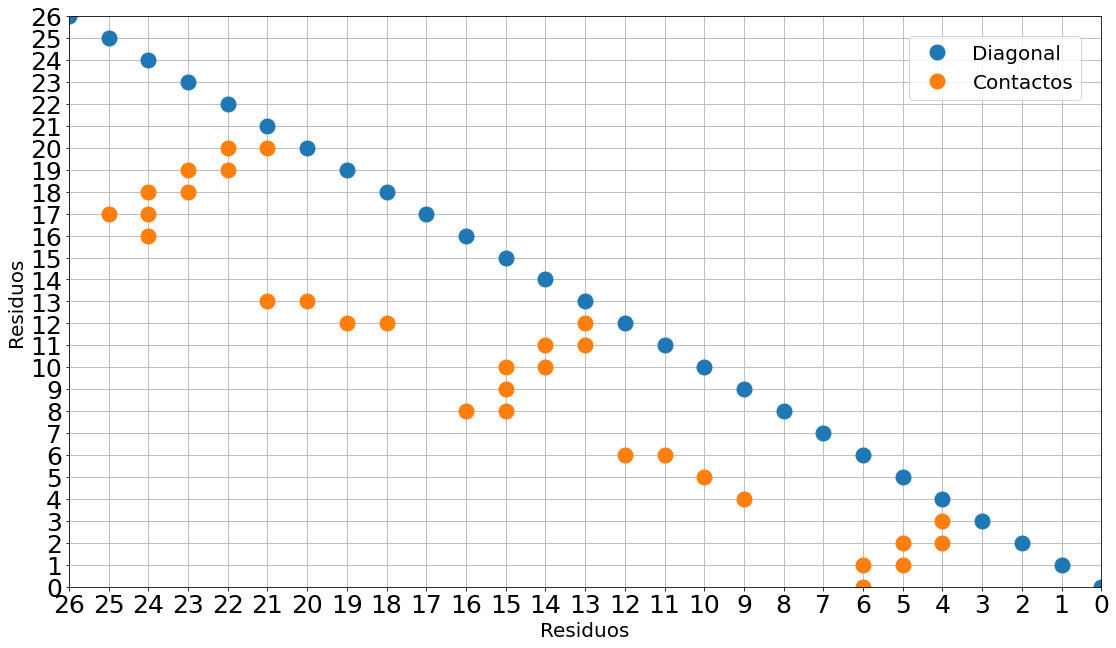
\includegraphics[scale=0.35]{meandro.jpg}
        \caption{Gráfico realizado de un meandro.}
    \end{figure}
    

    \np{Se realizó un gráfico donde se muestra la estructura de un meandro formado por tres hebras (ver gráfico del meandro).}
    

    \begin{figure}[h]
        % Reactive %
        \centering
        \begin{minipage}[b]{0.49\textwidth}
            \centering
          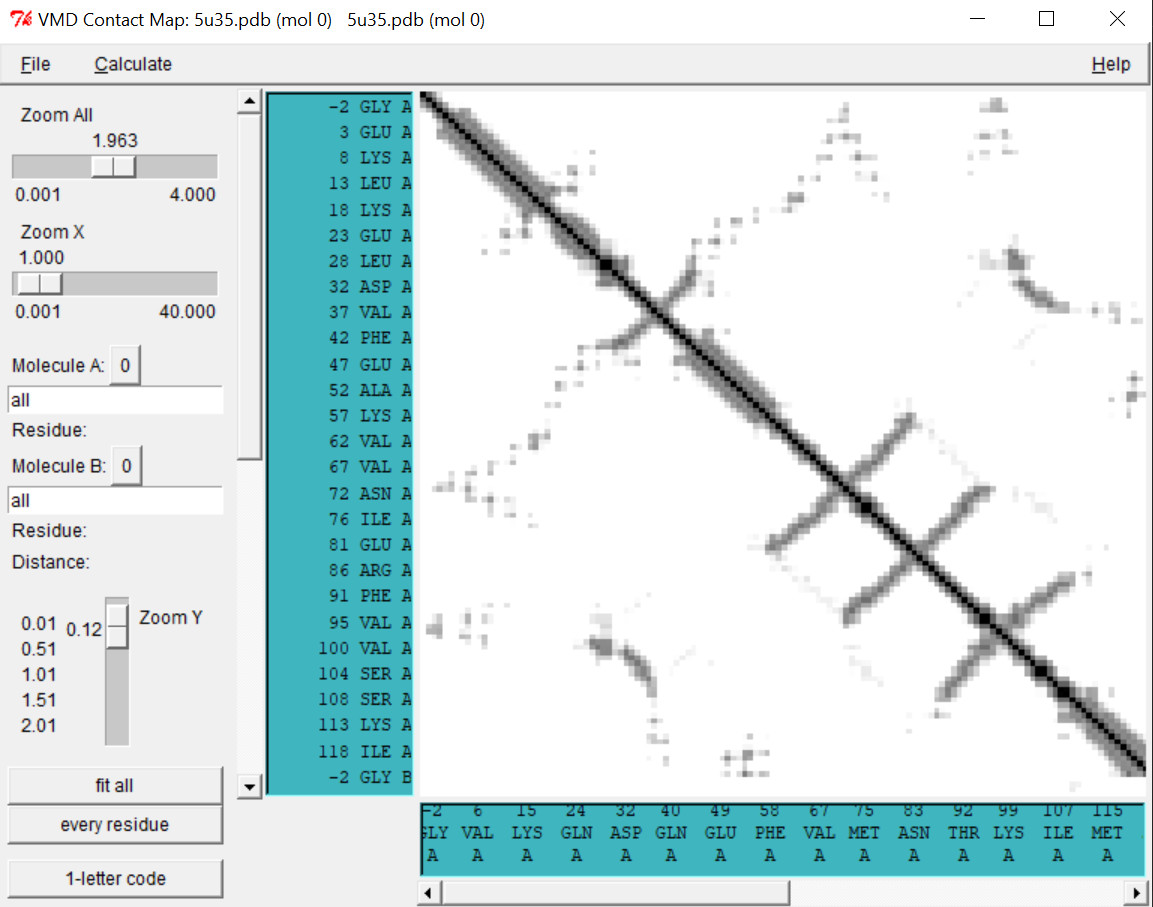
\includegraphics[scale=0.4,frame]{vmd.jpg}
          \caption{Gráfico de contacto calculado con VMD de 5U35.}
        \end{minipage}
        \begin{minipage}[b]{0.49\textwidth}
            \centering
          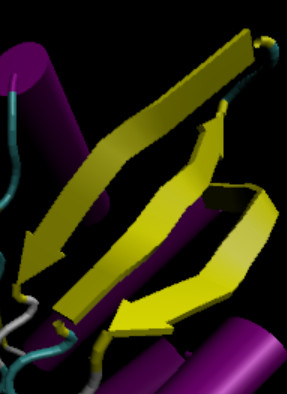
\includegraphics[scale=0.9,frame]{meandro3D.jpg}
          \caption{Meando 3D en 5U35.}
        \end{minipage}
    \end{figure}    

    \np{Posteriormente para corroborar que dicha estructura es cercana a un meandro real, se busco una proteína en el PDB que tuviera un meandro y se eligio la proteína 5U35, se uso el visualizador VMD para poder hacer el calculo de su mapa de contactos y buscar el meandro el cual se observa en la sigueinte figura, que son las tres diagonales paralelas entre si, estas las podemos ver de forma 3D representada en forma de caricatura en el lado derecho como las tres flechas antiparalelas.}

    
    





    % Pregunta 6 %
    
    \np{6) Empleando los radios de 1.68  ̊A para el ión Na+ y 1.94  ̊A para el ión Cl− calcule la energía necesaria para colocar por separado a un ión sodio y un ión cloruro en el interior de una proteína (Dprot = 3.5D0). ¿Será necesario una mayor cantidad de energía si se desea colocar un ión potasio en el interior de la proteína? Fundamente su respuesta.}

    \np{Se calculo la autoenergia del ión $Na^+$ y $Cl^-$}

    \ec{
        E_{Na^{+}_{prot}}=\frac{(1.6022x10^{-19}C)^2}{2(3.5)(4\pi 8.885x10^{-12}C^2J^{-1}m^{-1})(1.68x10^{-10}m)}(\frac{6.022x10^{23}}{mol})(\frac{1kJ}{1000J})=117.73 kJ/mol
    }

    \ec{
        E_{Cl^{-}_{prot}}=\frac{(1.6022x10^{-19}C)^2}{2(3.5)(4\pi 8.885x10^{-12}C^2J^{-1}m^{-1})(1.94x10^{-10}m)}(\frac{6.022x10^{23}}{mol})(\frac{1kJ}{1000J})=101.95 kJ/mol
    }

    \np{El ión $K^+$ no requerirá más energía para estar dentro de la proteína que el ión de $Cl^-$, pero si más que el ión $Na^+$, esto es debido a que el radio del $K^+$ será mayor al de $Na^+$ y menor al del $Cl^-$ de acuerdo con las propiedades periodicas, esto implica que al tener un mayor radio que el $Na^+$ su valor de autoenergía sera menor, pero siendo todavia mayor al valor de la autoenergía del $Cl^-$ que possee el radio más grande entre los tres iones.}

    % Pregunta 7 %
    
    \np{7) Calcule el número de posibles hexapéptidos que se pueden construir sin imponer alguna restricción. ¿Cuántos pentapéptidos distintos se pueden construir si de los 20 amino ́ácidos sólo se emplean los amino ácidos polares? ¿Cuántos pentapéptidos distintos se pueden construir si de los 20 amino ́acidos sólo se emplean
    amino ácidos no polares? Indique en su hoja de respuesta los cálculos que realizó.}

    \np{Se calculan las permutaciones con $n^r$}

    \ec{\# hexapeptidos=20^6=64000000}
    \ec{\# pentapeptidos_{apolaresNoIonicos}=9^5=59049}
    \ec{\# pentapeptidos_{polaresNoIonicos}=4^5=1024}

    % Pregunta 8 %
    
    \np{8) Obtenga la ecuación para calcular el volumen de la cadena hidrocarbonada, empleando para ello las densidades del n-hexano (C6H14 ρ = 654.8 kg m−3, M = 86.18 g mol−1) y n-dodecano (C12H26, ρ = 748.7 kg m−3, M = 170.34 g mol−1).}

    \np{Se usan los datos de densidad para obtener el volumen por molécula.}

    \begin{center}
        \begin{tabular}{ |c|c|c|c|c|c|c| } 
            \hline
            Nombre & Densidad $(kg/m^3)$ & PM $(g/mol)$ & PM $(kg/mol)$ & Volumen $(m^3)$ & Volumen $(nm^3)$ & Nc \\ 
            \hline 
            n-hexano & 654.8 & 86.18 & 0.08618 & 2.19E-28 & 0.2185 & 6\\ 
            \hline 
            n-dodecano & 748.7 & 170.34 & 0.17034 & 3.78E-28 & 0.3778 & 12 \\ 
            \hline 
        \end{tabular}
    \end{center}

    \np{El volumen de cada hidrocarburo se calculó por medio de la siguiente ecuación.}

    \ec{v=\frac{PM}{\rho N_A}(1x10^{27}nm^3)}

    \np{Gráfico Volumen vs Número de carbonos.}

    \np{Y por medio de los dos puntos, se graficó una grafica de volumen vs Nc (número de carbonos), obteniendo los valores de m y b.}
    
    \begin{figure}[h!]
        % Reactive %
        \centering
        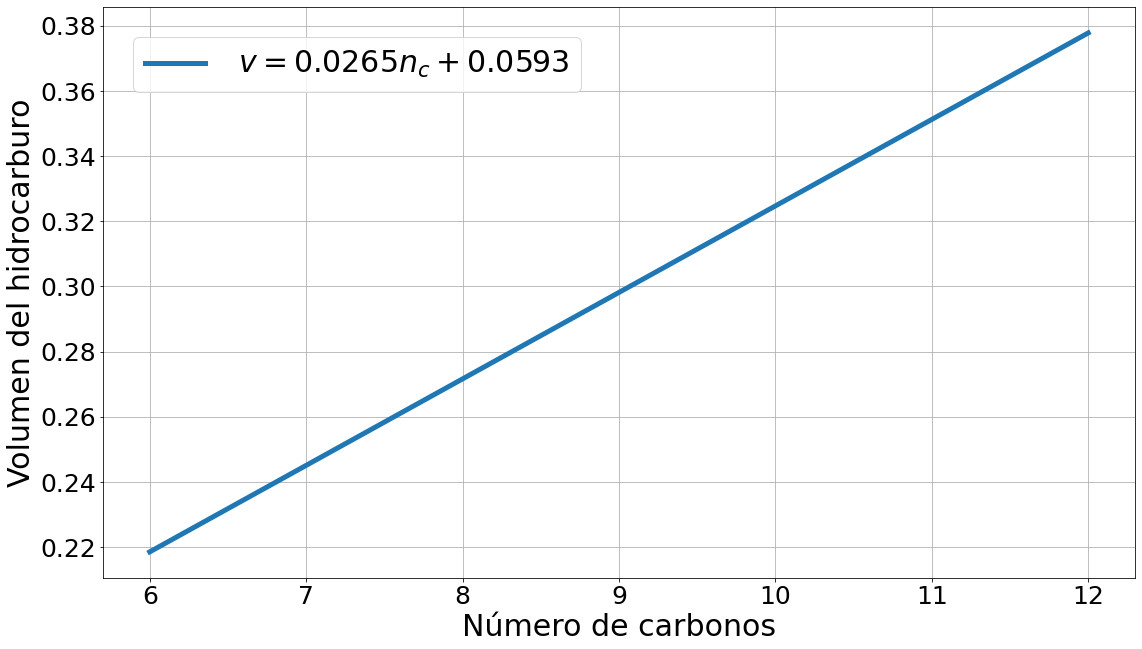
\includegraphics[scale=0.35]{volumen.jpg}
    \end{figure}
    
    \begin{center}
        \begin{tabular}{ |c|c| } 
            \hline
            m  & b   \\ 
            \hline 
            0.0265 & 0.0593  \\ 
            \hline 
        \end{tabular}
    \end{center}

    \np{La ecuación que describe el volumen de la cadena hidrocarbonada es \bt{v=0.0265Nc+0.0593} } 

    % Pregunta 9 %
    
    \np{9) El proceso de micelización es promovido por el efecto hidrofóbico. Estime el cambio en la energía libre de Gibbs (∆Gtrans) asociado con transferir un grupo metileno (–CH2–), de un medio acuoso al interior de la micela. Utilice para ello los valores de concentración micelar crítica (CMC) de etilenglicoles de alquilo tabulados en la tabla 1.}
  
    \begin{center}
        \begin{tabular}{ |c|c| } 
            \hline
            Surfactante  & CMC (mM)   \\ 
            \hline 
            $C_{10}H_{21}(OCH_2CH_2)_8OH$ & 1.0  \\ 
            \hline 
            $C_{12}H_{25}(OCH_2CH_2)_8OH$ & $7.1x10^-1$  \\ 
            \hline 
            $C_{14}H_{29}(OCH_2CH_2)_8OH$ & $9.0x10^-3$  \\ 
            \hline 
        \end{tabular}
    \end{center}

    \np{Se calcularon los valores de la energía libre del proceso de miceización donde se puede apreciar el cambio producido por la adición del grupo metilo.}

    \begin{figure}[h!]
        % Reactive %
        \centering
        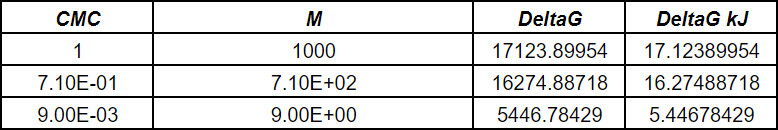
\includegraphics[scale=0.5]{delta.jpg}
    \end{figure}


\end{document}
%%%%%%%%%%%%%%%% END DOCUMENT %%%%%%%%%%%%%%%%